\documentclass[aspectratio=1610,t]{beamer}

\usepackage[english]{babel}
\usepackage{hyperref}
\usepackage{minted}
\usepackage{alltt}
\usepackage{amsmath}
\usepackage{graphicx}
\usepackage{xcolor}
\usepackage[utf-8]{inputenc}

\usetheme{metropolis}
\usemintedstyle{xcode}
\definecolor{codebg}{RGB}{247, 247, 246}
\setbeamercolor{background canvas}{bg=white}
\hypersetup{colorlinks,linkcolor=,urlcolor=orange}

\title{Lecture 4: Cargo and Iterators}
\date{March 22, 2022}
\author{Alexander Stanovoy}
\institute{alex.stanovoy@gmail.com}

\begin{document}

% ----------------------------------------------------------------- %

\begin{frame}
\maketitle
\end{frame}

% ----------------------------------------------------------------- %

\begin{frame}[fragile]
\frametitle{In this lecture}
\begin{itemize}
    \item Cargo and crates
    \item Modules
    \item Iterators
\end{itemize}
\end{frame}

% ----------------------------------------------------------------- %

\begin{frame}[c]
\centering\Huge\textbf{Cargo and crates}
\end{frame}

% ----------------------------------------------------------------- %

\begin{frame}[fragile]
\frametitle{Cargo}
Cargo is the Rust language package manager. It's one of the greatest things about Rust!

What Cargo does do?

\begin{itemize}
    \item Downloads and manages your dependencies.
    \item Compiles your packages.
    \item Makes distributable packages.
    \item And more!
\end{itemize}
\end{frame}

% ----------------------------------------------------------------- %

\begin{frame}[fragile]
\frametitle{Crate}
A crate is a compilation unit in Rust. It's like a package in other languages. An example of crate created by \texttt{cargo new --bin example} command:

\begin{verbatim}
    example
    ├── Cargo.lock
    ├── Cargo.toml
    └── src
    └── main.rs
\end{verbatim}

Packages can be uploaded to \href{https://crates.io}{crates.io}, the Rust community's crate registry. It makes them available to everyone, and users will have an opportunity to use your crate as a dependency at the manifest.
\end{frame}

% ----------------------------------------------------------------- %

\begin{frame}[fragile]
\frametitle{Crate}
A package is described using manifest file called \texttt{Cargo.toml}. Here's an example:

\begin{minted}{toml}
    [package]
    name = "example"
    version = "0.1.0"
    edition = "2021"

    [dependencies]
    clap = "3.1.0"
\end{minted}
\end{frame}

% ----------------------------------------------------------------- %

\begin{frame}[fragile]
\frametitle{Crate: \texttt{Cargo.toml}}
\texttt{Cargo.toml} consists of multiple entries.\footnote{\href{https://doc.rust-lang.org/cargo/reference/manifest.html#the-rust-version-field}{The Manifest Format}} Here's an example:

\begin{itemize}
    \item \texttt{[package]} has the meta information about package like name, version, authors, edition, compiler version, build scripts...
    \item \texttt{[dependencies]} describes dependencies of our package, their versions, needed features.
    \item \texttt{[features]} provides a mechanism to express conditional compilation and optional dependencies.
    \item \texttt{[profile.TYPE]} describes how to compile in different profiles: \texttt{dev}, \texttt{release}, \texttt{test} and \texttt{bench}.
    \item And more!
\end{itemize}
\end{frame}

% ----------------------------------------------------------------- %

\begin{frame}[fragile]
\frametitle{Crate}
There are multiple types of crates.\footnote{\href{https://doc.rust-lang.org/reference/linkage.html}{Linkage, The Rust Reference}}

\begin{itemize}
    \item \texttt{bin} - a runnable executable. It's default crate type
    \item \texttt{lib} - a ``compiler recommended'' Rust library.
    \item \texttt{dylib} - a dynamic Rust library.
    \item \texttt{staticlib} - a static system library.
    \item \texttt{cdylib} - a C dynamic library.
    \item \texttt{rlib} - a ``Rust library'' file.
    \item \texttt{proc-macro} - a procedural macros crate.
\end{itemize}

\texttt{bin} or \texttt{lib} types should be sufficient for all compilation needs.
\end{frame}

% ----------------------------------------------------------------- %

\begin{frame}[fragile]
\frametitle{Crate: versions}
In Cargo, versions of packages \textbf{must be changed} accordingly to Semantic Versioning (semver).\footnote{\href{https://semver.org}{Semantic Versioning 2.0.0}}

Given a version number \texttt{MAJOR.MINOR.PATCH}, increment the:

\begin{itemize}
    \item \texttt{MAJOR} version when you make incompatible API changes.
    \item \texttt{MINOR} version when you add functionality in a backwards compatible manner.
    \item \texttt{PATCH} version when you make backwards compatible bug fixes.
\end{itemize}
\end{frame}

% ----------------------------------------------------------------- %

\begin{frame}[fragile]
\frametitle{Crate: versions}
For instance, this version changes are legal:\footnote{\href{https://doc.rust-lang.org/cargo/reference/semver.html}{SemVer Compatibility}}

\begin{itemize}
    \item \texttt{1.3.7} -> \texttt{1.3.8} (bug fix).
    \item \texttt{1.5.5} -> \texttt{1.6.0} (added functionality).
    \item \texttt{1.7.2} -> \texttt{2.0.0} (major update, incompatible changes).
\end{itemize}

If your \texttt{MAJOR} version number is 0, Cargo will treat \texttt{MINOR} as \texttt{MAJOR} and \texttt{PATCH} as \texttt{MINOR}.
\end{frame}

% ----------------------------------------------------------------- %

\begin{frame}[fragile]
\frametitle{Crate: versions}
In \texttt{Cargo.toml}:

\begin{itemize}
    \item \texttt{\^{}1.2.3} - semver compatible (\texttt{< 2.0.0})
    \item \texttt{\~1.2.3} - only the last number is updated (\texttt{< 1.3.0})
    \item \texttt{1.2.*}
    \item \texttt{>= 1.2}
\end{itemize}

If your \texttt{MAJOR} version number is 0, Cargo will treat \texttt{MINOR} as \texttt{MAJOR} and \texttt{PATCH} as \texttt{MINOR}.
\end{frame}

% ----------------------------------------------------------------- %

\begin{frame}[fragile]
\frametitle{\texttt{Cargo.toml} vs \texttt{Cargo.lock}}
\begin{itemize}
    \item \texttt{Cargo.toml} is about describing your dependencies in a broad sense, and is written by you.
    \item \texttt{Cargo.lock} contains exact information about your dependencies. It is maintained by Cargo and should not be manually edited.
\end{itemize}

\visible<2->{
    The purpose of a \texttt{Cargo.lock} lockfile is to describe the state of the world at the time of a successful build.
}

\visible<3->{
    This property is the most desirable for packages that are at the very end of the dependency chain (binaries).
}

\visible<4->{
    But the library is not only used by the library developers, but also any downstream consumers of the library. Libraries specify semver requirements for their dependencies but cannot see the full picture. Only end products like binaries have a full picture to decide what versions of dependencies should be used.
}
\end{frame}

% ----------------------------------------------------------------- %

\begin{frame}[fragile]
\frametitle{\texttt{cargo-edit}}
\begin{itemize}
    \item \texttt{cargo add foo} - add the latest version of library \texttt{foo} to \texttt{Cargo.toml}.
    \item \texttt{cargo rm foo} - remove library \texttt{foo} from \texttt{Cargo.toml}.
    \item \texttt{cargo upgrade} - upgrade all dependencies versions in \texttt{Cargo.toml} to latest.
\end{itemize}

To install, run \texttt{cargo install cargo-edit}
\end{frame}

% ----------------------------------------------------------------- %

\begin{frame}[fragile]
\frametitle{Rust versions}
Rust version changes accordingly to semver, but how this exactly works?

\begin{itemize}
    \item<1-> Before version 1.0, as a new product, Rust changed frequently and hadn't given any guarantees about how your code will be compiled in future releases.
    \item<2-> After the release of 1.0, Rust started following one of the variations of ``stability without stagnation'' model, first introduced in web browsers.
    \item<3-> New work lands directly in the master branch.
    \item<4-> Each day, the last successful build from the master becomes the new nightly release.
    \item<5-> Every six weeks, a beta branch is created from the current state of the master, and the previous beta is promoted to be the new stable release.
\end{itemize}
\end{frame}

% ----------------------------------------------------------------- %

\begin{frame}[fragile]
\frametitle{Rust versions}
Rust version changes accordingly to semver, but how this exactly works?

\begin{itemize}
    \item<1-> In short, there are three release channels - nightly, beta, and stable - with regular, frequent promotions from one channel to the next.
    \item<2-> New features and new APIs will be flagged as unstable via feature gates and stability attributes respectively. Unstable features and standard library APIs will only be available on the nightly branch, and only if you explicitly ``opt-in'' to the instability.
    \item<3-> But sometimes, make small changes to the language that are not backward compatible. The most obvious example is introducing a new keyword, which would invalidate variables with the same name.
    \item<4-> For instance, before 2018 there were no \texttt{async} and \texttt{await} keywords.
    \item<5-> When the release is about to break code, it becomes a part of the new edition. The choice of edition is made in \texttt{Cargo.toml} for a crate.
\end{itemize}
\end{frame}

% ----------------------------------------------------------------- %

\begin{frame}[fragile]
\frametitle{Rust versions}
Rust version changes accordingly to semver, but how this exactly works?

\begin{itemize}
    \item<1-> This ensures that the decision to migrate to a newer edition is a ``private one'' that the crate can make without affecting your downstream crates.
    \item<2-> To automate migration, there's \texttt{cargo fix --edition} command.
    \item<3-> For example, when migrating to Rust 2018, it changes anything named async to use the equivalent raw identifier syntax: \texttt{r\#async}.
\end{itemize}
\end{frame}

% ----------------------------------------------------------------- %

\begin{frame}[fragile]
\frametitle{Features}
Cargo ``features'' provide a mechanism to express conditional compilation and optional dependencies.

\begin{minted}{toml}
    [features]
    bmp = []
    png = []
    ico = ["bmp", "png"]
    default = ["ico"]
\end{minted}

\begin{minted}{rust}
    #[cfg(feature = "ico")]
    pub mod ico;
\end{minted}
\end{frame}

% ----------------------------------------------------------------- %

\begin{frame}[fragile]
\frametitle{Features}
\begin{minted}{toml}
    [dependencies]
    reqwest = {
        version = ">= 0.11.9",
        features = ["blocking", "multipart"]
    }
\end{minted}
\end{frame}

% ----------------------------------------------------------------- %

\begin{frame}[fragile]
\frametitle{Features}
The crate is compiled with all features needed for all dependencies.

\textbf{Important}: Features are \textbf{additive}!

\textbf{Question}: What can be wrong if your feature appeared to be non-additive?

\visible<2->{
    Rust is frequently used for embedded programming. Some crates provide the \texttt{no\_std} feature to enable usage of the crate in.
}

\visible<3->{
    As you may notice, \texttt{no\_std} is \textbf{non-additive}, since \texttt{std} can do the same and even more.
}

\visible<4->{
 I  f there will be two crates depending on this crate with \texttt{no\_std} enabled in one crate and disabled in another, Cargo will compile with this crate with \texttt{no\_std}, leading to errors!
}
\end{frame}

% ----------------------------------------------------------------- %

\begin{frame}[fragile]
\frametitle{Features}
It's a common practice to implement some additional features as a crate feature.

\visible<2->{
    Such common that \href{https://rust-lang.github.io/api-guidelines/about.html}{Rust API guidelines} book suggests to implement \texttt{Serialize} and \texttt{Deserialize} traits from crate \texttt{serde}.
}

\visible<3->{
    Features give users a chance to conditionally opt-in to additional features rather than compiling them all the time.
}
\end{frame}

% ----------------------------------------------------------------- %

\begin{frame}[fragile]
\frametitle{\texttt{rustc}}
As you can see, we don't need to even know something about \texttt{rustc}! (expect version, of course)

This is one of the cool things about Cargo.

A detailed discussion of it is not part of this lecture.
\end{frame}

% ----------------------------------------------------------------- %

\begin{frame}[c]
\centering\Huge\textbf{Modules}
\end{frame}

% ----------------------------------------------------------------- %

\begin{frame}[fragile]
\frametitle{Modules}
In C language, there are no namespaces. Combination of this and how \texttt{\#include} preprocessor directive works results in name pollution. There are no good ways to solve this problem.\footnote{At least no direct solutions.}

\visible<2->{
    In C++, name pollution is solved using namespaces. Namespaces are a pretty simple and practical solution.
}

\visible<3->{
    What we'll do in Rust to prevent name pollution and use multiple files in the project?
}
\end{frame}

% ----------------------------------------------------------------- %

\begin{frame}[fragile]
\frametitle{Modules}
\begin{minted}[fontsize=\small]{rust}
    mod one {
        mod nested {
            mod nested2 {
                struct Foo { /* ... */ }
            }
            enum Count { /* ... */ }
        }
        trait MyTrait { /* ... */ }
    }
    mod two {
        struct Bar { /* ... */ }
        fn use_me() { /* ... */ }
    }
\end{minted}

\texttt{mod} keyword defines a module. Modules are used to control the visibility of declarations inside it and to prevent namespace pollution.
\end{frame}

% ----------------------------------------------------------------- %

\begin{frame}[fragile]
\frametitle{Modules}
We can use the \texttt{use\_me} using full path:

\begin{minted}{rust}
    two::use_me();
\end{minted}
\end{frame}

% ----------------------------------------------------------------- %

\begin{frame}[fragile]
\frametitle{Modules}
We can use the \texttt{use\_me} using full path:

\begin{minted}{rust}
    two::use_me();
\end{minted}

But unlike in C++, this code won't compile:

\begin{minted}{rust}
error[E0603]: function `use_me` is private
  --> src/main.rs:16:12
   |
16 | two::use_me();
   |      ^^^^^^ private function
\end{minted}
\end{frame}

% ----------------------------------------------------------------- %

\begin{frame}[fragile]
\frametitle{Modules}
\begin{minted}[fontsize=\small]{rust}
    mod one {
        mod nested {
            mod nested2 {
                struct Foo { /* ... */ }
            }
            enum Count { /* ... */ }
        }
        trait MyTrait { /* ... */ }
    }
    mod two {
        struct Bar { /* ... */ }
        pub fn use_me() { /* ... */ }
    }
\end{minted}

We'll use \texttt{pub} keyword. It means ``make it private for all parent modules''.
\end{frame}

% ----------------------------------------------------------------- %

\begin{frame}[fragile]
\frametitle{Modules}
Next, we'll create \texttt{Foo} structure:

\begin{minted}{rust}
    let _ = one::nested::nested2::Foo {};
\end{minted}
\end{frame}

% ----------------------------------------------------------------- %

\begin{frame}[fragile]
\frametitle{Modules}
Next, we'll create \texttt{Foo} structure:

\begin{minted}{rust}
    let _ = one::nested::nested2::Foo {};
\end{minted}

We'll find out our module is private!

\begin{minted}{rust}
error[E0603]: module `nested` is private
  --> src/main.rs:16:18
   |
16 | let _ = one::nested::nested2::Foo {};
   |              ^^^^^^ private module
\end{minted}
\end{frame}

% ----------------------------------------------------------------- %

\begin{frame}[fragile]
\frametitle{Modules}
So, unlike in C++ namespaces, Rust modules are private by default!

But why compiler asked to make public the declaration of \texttt{nested}? And in the previous case - \texttt{two}?

\visible<2->{
    Because \texttt{one} and \texttt{two} are the part of our current module called \textbf{the root module}. We don't need to have rights to use the declarations in our current module - everything is public for us.
}

\visible<3->{
    Let's make \texttt{nested} public. Then we'll get compiler errors since \texttt{nested2} and \texttt{Foo} are private and make them public them too.
}
\end{frame}

% ----------------------------------------------------------------- %

\begin{frame}[fragile]
\frametitle{Modules}
\begin{minted}[fontsize=\small]{rust}
    mod one {
        pub mod nested {
            pub mod nested2 {
                pub struct Foo { /* ... */ }
            }
            enum Count { /* ... */ }
        }
        trait MyTrait { /* ... */ }
    }
    mod two {
        struct Bar { /* ... */ }
        pub fn use_me() { /* ... */ }
    }
\end{minted}
\end{frame}

% ----------------------------------------------------------------- %

\begin{frame}[fragile]
\frametitle{Modules}
\begin{minted}[fontsize=\small]{rust}
    mod one {
        pub mod nested {
            mod nested2 { // No 'pub'
                pub struct Foo { /* ... */ }
            }
            enum Count { /* ... */ }
        }
        trait MyTrait { /* ... */ }
    }
    mod two {
        struct Bar { /* ... */ }
        pub fn use_me() { /* ... */ }
    }
\end{minted}

Note that the following code won't make \texttt{Foo} available since \texttt{nested2} is private for us.
\end{frame}

% ----------------------------------------------------------------- %

\begin{frame}[fragile]
\frametitle{Modules}
\begin{minted}[fontsize=\small]{rust}
    mod one {
        pub mod nested {
            pub mod nested2 {
                pub struct Foo { bar: two::Bar }
            }
            enum Count { /* ... */ }
        }
        trait MyTrait { /* ... */ }
    }
    mod two {
        struct Bar { /* ... */ }
        pub fn use_me() { /* ... */ }
    }
\end{minted}

Next, we'll try to add a field \texttt{bar} of type \texttt{two::Bar} to \texttt{one::nested::nested2::Foo}.
\end{frame}

% ----------------------------------------------------------------- %

\begin{frame}[fragile]
\frametitle{Modules}
\begin{minted}[fontsize=\small]{rust}
error[E0433]: failed to resolve: use of undeclared crate
              or module `two`
  --> src/main.rs:4:35
   |
 4 | pub struct Foo { bar: two::Bar }
   |                       ^^^ use of undeclared crate or module `two`
\end{minted}

Why did this happen?

\visible<2->{
    By default, paths are relative. To make them absolute, we should use \texttt{crate} keyword (remember the path \texttt{/} in Unix systems?). In this case, our path will always start from the root module, not from the current module.
}
\end{frame}

% ----------------------------------------------------------------- %

\begin{frame}[fragile]
\frametitle{Modules}
\begin{minted}[fontsize=\small]{rust}
    mod one {
        pub mod nested {
            pub mod nested2 {
                pub struct Foo { bar: crate::two::Bar }
            }
            enum Count { /* ... */ }
        }
        trait MyTrait { /* ... */ }
    }
    mod two {
        // Note the 'pub'
        pub struct Bar { /* ... */ }
        pub fn use_me() { /* ... */ }
    }
\end{minted}

Since \texttt{Bar} is private in module \texttt{two}, we should use \texttt{pub} here too.
\end{frame}

% ----------------------------------------------------------------- %

\begin{frame}[fragile]
\frametitle{Modules}
Note that now we cannot construct \texttt{Foo} because it's \texttt{bar} field is private!

\begin{minted}{rust}
    let _ = one::nested::nested2::Foo { bar: two::Bar {} };
\end{minted}

\begin{minted}[fontsize=\small]{rust}
error[E0451]: field `bar` of struct `Foo` is private
  --> src/main.rs:17:41
   |
17 |let _ = one::nested::nested2::Foo { bar: two::Bar {} };
   |                                    ^^^^^^^^^^^^^^^^ private field
\end{minted}

In Rust, fields of structs are private by default and available only for the current module. It's the cause why you cannot access fields of, for instance, \texttt{Vec}. To fix this, you should make the field public.

But, of course, do not do this without reason: it's much better to implement type constructors and getters.
\end{frame}

% ----------------------------------------------------------------- %

\begin{frame}[fragile]
\frametitle{Modules}
\begin{minted}[fontsize=\small]{rust}
    mod one {
        pub mod nested {
            pub mod nested2 {
                pub struct Foo { pub bar: crate::two::Bar }
            }
        enum Count { /* ... */ }
        }
        trait MyTrait { /* ... */ }
    }
    mod two {
        pub struct Bar { /* ... */ }
        pub fn use_me() { /* ... */ }
    }
\end{minted}
\end{frame}

% ----------------------------------------------------------------- %

\begin{frame}[fragile]
\frametitle{Modules}
\begin{minted}[fontsize=\small]{rust}
    mod one {
        pub mod nested {
            pub mod nested2 {
                pub struct Foo { bar: crate::two::Bar }
            }
            pub enum Count { Example(nested2::Foo) }
        }
        trait MyTrait { /* ... */ }
    }
    mod two {
        pub struct Bar { /* ... */ }
        pub fn use_me() { /* ... */ }
    }
\end{minted}

Let's add an enumeration variant to count and make it public as usual.
\end{frame}

% ----------------------------------------------------------------- %

\begin{frame}[fragile]
\frametitle{Modules}
Using the enumeration:

\begin{minted}{rust}
    let bar = two::Bar {};
    let foo = one::nested::nested2::Foo { bar };
    let example = one::nested::Count::Example(foo);
\end{minted}

Unlike in \texttt{struct}, all enumuration variants are available if the \texttt{enum} is available.
\end{frame}

% ----------------------------------------------------------------- %

\begin{frame}[fragile]
\frametitle{Modules}
\begin{minted}[fontsize=\small]{rust}
    mod one {
        pub mod nested {
            pub mod nested2 {
                pub struct Foo { bar: crate::two::Bar }
                impl crate::one::MyTrait for Foo {}
            }
            pub enum Count { Example(nested2::Foo) }
        }
        trait MyTrait { /* ... */ }
    }
    mod two {
        pub struct Bar { /* ... */ }
        pub fn use_me() { /* ... */ }
    }
\end{minted}

We want to implement \texttt{MyTrait} for \texttt{Foo}. It's done pretty easily. In Rust, we don't need an object to be \texttt{pub} when it's defined in one of the ancestor modules.
\end{frame}

% ----------------------------------------------------------------- %

\begin{frame}[fragile]
\frametitle{Modules}
\begin{minted}[fontsize=\small]{rust}
    mod one {
        pub mod nested {
            pub mod nested2 {
                pub struct Foo { bar: super::super::super::two::Bar }
                impl super::super::MyTrait for Foo {}
            }
            pub enum Count { Example(nested2::Foo) }
        }
        trait MyTrait { /* ... */ }
    }
    mod two {
        pub struct Bar { /* ... */ }
        pub fn use_me() { /* ... */ }
    }
\end{minted}

We can also use \texttt{super} keyword (remember the \texttt{..} on Unix?). Just for example, the declaration of field \texttt{bar} is also changed.
\end{frame}

% ----------------------------------------------------------------- %

\begin{frame}[fragile]
\frametitle{Modules}
\begin{minted}[fontsize=\small]{rust}
    mod one {
        pub mod nested {
            pub mod nested2 {
                pub struct Foo { bar: crate::two::Bar }
            }
            impl crate::one::MyTrait for nested2::Foo {}
            impl nested2::Foo {}
            pub(self) enum Count { Example(nested2::Foo) }
        }
        trait MyTrait { /* ... */ }
    }
    mod two {
        pub struct Bar { /* ... */ }
        pub fn use_me() { /* ... */ }
    }
\end{minted}

We can write \texttt{impl} where we want! (But please, don't do this)
\end{frame}

% ----------------------------------------------------------------- %

\begin{frame}[fragile]
\frametitle{Coherence}
\begin{minted}[fontsize=\small]{rust}
    mod one {
        pub mod nested {
            pub mod nested2 {
                pub struct Foo { bar: crate::two::Bar }
                impl crate::one::MyTrait for Foo {}
            }
            impl crate::one::MyTrait for nested2::Foo {}
            pub(self) enum Count { Example(nested2::Foo) }
        }
        trait MyTrait { /* ... */ }
    }
    mod two {
        pub struct Bar { /* ... */ }
        pub fn use_me() { /* ... */ }
    }
\end{minted}

Ok, I want multiple implementations of the trait in different modules.
\end{frame}

% ----------------------------------------------------------------- %

\begin{frame}[fragile]
\frametitle{Coherence}
\begin{minted}[fontsize=\small]{rust}
error[E0119]: conflicting implementations of trait `one::MyTrait`
              for type `one::nested::nested2::Foo`
 --> src/main.rs:8:9
  |
5 | impl crate::one::MyTrait for Foo {}
  | -------------------------------- first implementation here
 ...
8 | impl crate::one::MyTrait for nested2::Foo {}
  | ^^^^^^^^^^^^^^^^^^^^^^^^^^^^^^^^^^^^^^^^^ conflicting
  |                                           implementation for
  |                                           `/* */::Foo`
\end{minted}
\end{frame}

% ----------------------------------------------------------------- %

\begin{frame}[fragile]
\frametitle{Coherence}
\begin{itemize}
    \item<1-> Rust must guarrantie that there's only one implementation of trait for every object.
    \item<2-> More generally, there's \textit{coherence} property: for any given type and method, there is only ever one correct choice for which implementation of the method to use for that type.
    \item<3-> Consider what would happen if we could write own implementation of the \texttt{Display} trait for the \texttt{bool} type from the standard library. Now, for any code that tries to print a \texttt{bool} value and includes my crate, the compiler won't know whether to pick the implementation I wrote or the one from the standard library. Neither choice is correct or better than the other, and the compiler obviously cannot choose randomly.
\end{itemize}
\end{frame}

% ----------------------------------------------------------------- %

\begin{frame}[fragile]
\frametitle{Coherence}
\begin{itemize}
    \item<1-> Rust must guarrantie that there's only one implementation of trait for every object.
    \item<2-> More generally, there's \textit{coherence} property: for any given type and method, there is only ever one correct choice for which implementation of the method to use for that type.
    \item<3-> Consider what would happen if we could write own implementation of the \texttt{Display} trait for the \texttt{bool} type from the standard library. Now, for any code that tries to print a \texttt{bool} value and includes my crate, the compiler won't know whether to pick the implementation we wrote or the one from the standard library. Neither choice is correct or better than the other, and the compiler obviously cannot choose randomly.
\end{itemize}
\end{frame}

% ----------------------------------------------------------------- %

\begin{frame}[c,fragile]
\frametitle{Coherence}
\begin{tabular}{cl} 
\begin{tabular}{c}
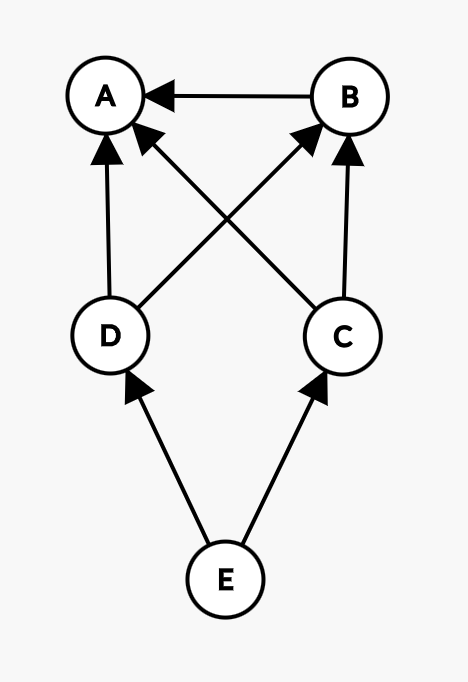
\includegraphics[height=5cm, width=3.5cm]{images/crates.png}
\end{tabular}
& \begin{tabular}{l}
    \parbox{0.6\linewidth}{
    \begin{itemize}
        \item<1-> Or the following: we've got crates \texttt{A} and \texttt{B}, in \texttt{A} there's trait, and in \texttt{B} there's a type. \texttt{B} depends on \texttt{A}. We want to use both of them as dependencies in the crate \texttt{C}. Also, there's crate \texttt{D} that depends on both \texttt{A} and \texttt{B}.
        \item<2-> Let's implement a trait from \texttt{A} for structure from \texttt{B} in \texttt{C} and \texttt{D}.
        \item<3-> In \texttt{E}, we have two implementations of trait!
    \end{itemize}
    }
\end{tabular} \\
\end{tabular}
\end{frame}

% ----------------------------------------------------------------- %

\begin{frame}[fragile]
\frametitle{Orphan rule}
To make sure the compiler will see only one implementation, there's \textit{orphan rule}.

Simply stated, the orphan rule says that you can implement a trait for a type only if the trait or the type is local to your crate (not module!).

In our example, we'll be able to implement a trait for type only in crate \texttt{B}.

In this rule, there are some exceptions.
\end{frame}

% ----------------------------------------------------------------- %

\begin{frame}[fragile]
\frametitle{Orphan rule: Blanket Implementations}
Remember: this is a \textit{blanket implementation}.

\begin{minted}{rust}
    impl<T> MyTrait for T where T: Something { /* ... */ }
\end{minted}

Only the crate that defines a trait is allowed to write a blanket implementation!

\textbf{Adding a blanket implementation to an existing trait is considered a breaking change}. If it were not, a downstream crate that contained \texttt{impl MyTrait for Foo} could suddenly stop compiling just because you update the crate that defines \texttt{MyTrait} with an error about a conflicting implementation.
\end{frame}

% ----------------------------------------------------------------- %

\begin{frame}[fragile]
\frametitle{Orphan rule: Fundamental Types}
Some types are so essential that it's necessary to allow anyone to implement traits on them.

These types currently include \texttt{\&}, \texttt{\&mut}, and \texttt{Box}. For the purposes of the orphan rule, fundamental types are erased before the orphan rule is checked.

\begin{minted}{rust}
    impl IntoIterator for &MyType { /* ... */ }
\end{minted}

With just the orphan rule, this implementation would not be permitted since it implements a foreign trait for a foreign type - \texttt{IntoIterator} and \texttt{\&} both come from the standard library.

\textbf{Note}: In standard library this types are marked by \texttt{\#[fundamental]} attribute.
\end{frame}

% ----------------------------------------------------------------- %

\begin{frame}[fragile]
\frametitle{Orphan rule: Covered Implementations}
There are some limited cases where we want to allow implementing a foreign trait for a foreign type, which the orphan rule does not normally allow:

\begin{minted}{rust}
    impl From<MyType> for Vec<i32> { /* ... */ }
\end{minted}

Here, the \texttt{From} trait is foreign, as is the \texttt{Vec} type.

Given \texttt{impl<P1..Pn> ForeignTrait<T1..Tm> for T0} is allowed only if at least one \texttt{Ti} is a local type and no \texttt{T} before the first such \texttt{Ti} is one of the generic types \texttt{P1..Pn}:

Generic type parameters (\texttt{P1..Pn}) are allowed to appear in \texttt{T0..Ti} as long as they are covered by some intermediate type. A \texttt{T} is covered if it appears as a type parameter to some other type (like \texttt{Vec<T>}), but not if it stands on its own (just \texttt{T}) or just appears behind a fundamental type like \texttt{\&T}.
\end{frame}

% ----------------------------------------------------------------- %

\begin{frame}[fragile]
\frametitle{Orphan rule: Covered Implementations}
A clarification example:

\begin{minted}[fontsize=\small]{rust}
    // 'X, Y, .., Z' - some generics
    // 'A, B, .., C' - some local types
    impl<X, Y, .., Z> ForeignTrait<u32, A, B, Vec<X>, C> for Vec<i32> {
        /* ... */
    }
\end{minted}
\end{frame}


% ----------------------------------------------------------------- %

\begin{frame}[fragile]
\frametitle{Orphan rule: Covered Implementations}
Note that:

\begin{minted}{rust}
    impl<T> ForeignTrait<LocalType, T> for ForeignType {}
\end{minted}

Is valid, but:

\begin{minted}{rust}
    impl<T> ForeignTrait<T, LocalType> for ForeignType {}
\end{minted}

Is not! Without ``generic comes after local'' rule, we could the code above, and another crate could write:

\begin{minted}{rust}
    impl<T> ForeignTrait<TheirType, T> for ForeignType {}
\end{minted}

And a conflict would arise only when the two crates were brought together. The orphan rule requires that your local type come before the type parameter.
\end{frame}

% ----------------------------------------------------------------- %

\begin{frame}[fragile,c]
\frametitle{Modules}
\begin{minted}[fontsize=\small]{rust}
    // Note the 'pub'
    pub mod one {
        pub mod nested {
            pub mod nested2 {
                pub(crate) struct Foo { bar: crate::two::Bar }
                impl crate::one::MyTrait for Foo {}
            }
            pub(self) enum Count { Example(nested2::Foo) }
        }
        trait MyTrait { /* ... */ }
    }
\end{minted}

Imagine we've put this in \texttt{lib.rs} file and published our crate. Since we added a \texttt{pub} keyword before \texttt{one}, and \texttt{one} is in our root module, everything inside became accessible for foreign crates. We don't want users to access \texttt{Foo}. One of the ways it to add \texttt{pub(crate)} visibility to \texttt{Foo}. Works just like \texttt{pub}, but only in our crate.
\end{frame}

% ----------------------------------------------------------------- %

\begin{frame}[fragile]
\frametitle{Modules}
\begin{minted}[fontsize=\small]{rust}
 pub mod one {
    pub mod nested {
        pub mod nested2 {
            pub(super) struct Foo { bar: crate::two::Bar }
            impl crate::one::MyTrait for Foo {}
        }
        pub(self) enum Count { Example(nested2::Foo) }
    }
    trait MyTrait { /* ... */ }
 }
\end{minted}

If we don't use \texttt{Foo} in any other modules than \texttt{nested2} and \texttt{nested}, there's \texttt{pub(super)} to help. It makes object available only for current module and parent module.
\end{frame}

% ----------------------------------------------------------------- %

\begin{frame}[fragile]
\frametitle{Modules}
\begin{minted}[fontsize=\small]{rust}
 pub mod one {
    pub mod nested {
        pub mod nested2 {
            pub(in crate::one::nested) struct Foo { /* ... */ }
            impl crate::one::MyTrait for Foo {}
        }
        pub(self) enum Count { Example(nested2::Foo) }
    }
    trait MyTrait { /* ... */ }
 }
\end{minted}

We can use \texttt{pub(in PATH)} to make the object visible for all ancestors from specified. For instance, in this example, we won't see \texttt{Foo} in module \texttt{one}, but all other ancestor modules will.
\end{frame}

% ----------------------------------------------------------------- %

\begin{frame}[fragile]
\frametitle{\texttt{use} keyword}
The availability of the type and definition is not the same in Rust. When you make the function public, you must have your input and output types to be at least with the same availability.

The same applies to enumerations and structures.

\begin{minted}{rust}
    mod A {
        pub mod B {
            enum Private { X }
            pub fn MyFunc(x: Private) {}
            pub enum MyEnum { Variant(Private) }
            pub struct S { pub x: Private }
        }
    }
\end{minted}
\end{frame}

% ----------------------------------------------------------------- %

\begin{frame}[fragile]
\frametitle{\texttt{use} keyword}
\begin{minted}[fontsize=\small]{rust}
error[E0446]: private type `Private` in public interface
 --> src/main.rs:4:9
  |
3 | enum Private { X }
  | ------------ `Private` declared as private
4 | pub fn MyFunc(x: Private) {}
  | ^^^^^^^^^^^^^^^^^^^^^^^^^ can't leak private type
6 | pub struct S { pub x: Private }
  | ^^^^^^^^^^^^^^ can't leak private type
\end{minted}
\end{frame}

% ----------------------------------------------------------------- %

\begin{frame}[fragile]
\frametitle{\texttt{use} keyword}
\begin{minted}[fontsize=\small]{rust}
warning: private type `Private` in public interface (error E0446)
 --> src/main.rs:5:35
  |
5 | pub enum MyEnum { Variant(Private) }
  |                           ^^^^^^^
  |
 = note: `#[warn(private_in_public)]` on by default
 = warning: this was previously accepted by the compiler
 but is being phased out; it will become a hard error in
 a future release!
 = note: for more information, see issue #34537
 <https://github.com/rust-lang/rust/issues/34537>
\end{minted}
\end{frame}

% ----------------------------------------------------------------- %

\begin{frame}[fragile]
\frametitle{\texttt{use} keyword}
In C++, this code will compile just fine:

\begin{minted}[fontsize=\small]{cpp}
    class Class {
    private:
        struct Example {};
    
    public:
        static Example get() {
            return Example {};
        }
    };
    
    int main() {
        auto example = Class::get();
    }
\end{minted}
\end{frame}

% ----------------------------------------------------------------- %

\begin{frame}[fragile,c]
\frametitle{Modules and files}
We've already seen \texttt{super} and \texttt{crate} keywords, and they was pretty close to Unix paths. It's not a coincidence! This code...

\begin{minted}[fontsize=\small]{rust}
    mod one {
        pub mod nested {
            pub mod nested2 {
                pub struct Foo { bar: crate::two::Bar }
            }
            impl crate::one::MyTrait for nested2::Foo {}
            pub(self) enum Count { Example(nested2::Foo) }
        }
        trait MyTrait { /* ... */ }
    }
    mod two {
        pub struct Bar { /* ... */ }
        pub fn use_me() { /* ... */ }
    }
\end{minted}
\end{frame}

% ----------------------------------------------------------------- %

\begin{frame}[fragile]
\frametitle{Modules and files}
...Translates to this in filesystem!

\small\begin{verbatim}
    .
    ├── Cargo.toml
    └── src
        ├── lib.rs
        ├── one
        │   ├── mod.rs
        │   └── nested
        │       ├── mod.rs
        │       └── nested2.rs
        └── two.rs
\end{verbatim}
\end{frame}

% ----------------------------------------------------------------- %

\begin{frame}[fragile]
\frametitle{Modules and files}
Well, how this works?

\begin{itemize}
    \item<1-> Every file is a module. The path to this file including it's name is module name. Exceptions - \texttt{main.rs}, \texttt{lib.rs} and \texttt{mod.rs} files. Their names ``empty'' for Rust, and everything inside them is in the root module.
    \item<2-> For instance, \texttt{two.rs} file has path \texttt{crate::two}, and \texttt{nested2.rs} - \texttt{crate::one::nested::nested2}.
\end{itemize}
\end{frame}

% ----------------------------------------------------------------- %

\begin{frame}[fragile]
\frametitle{Modules and files}
Well, how this works?

\begin{itemize}
    \item<1-> When your module contains not only code but also other modules, you should create a directory. Inside it, you'll have \texttt{mod.rs} file in which declarations will have the path of the directory.
    \item<2-> For instance, code inside \texttt{mod.rs} in \texttt{nested} have module path of \texttt{crate::one::nested}.
\end{itemize}
\end{frame}

% ----------------------------------------------------------------- %

\begin{frame}[fragile]
\frametitle{Modules and files}
Well, how this works?

\begin{itemize}
    \item<1-> Modules aren't available to the whole program by default! To include module in file, use \texttt{pub mod MODULE;} syntax: because there's no \texttt{\{\}}, Rust finds out it's not a declaration but usage of the module. File \texttt{src/one/mod.rs} contains:

    \begin{minted}{rust}
    pub mod nested;
    trait MyTrait { /* ... */ }
    \end{minted}
\end{itemize}
\end{frame}

% ----------------------------------------------------------------- %

\begin{frame}[fragile]
\frametitle{\texttt{use} keyword}
There's one convenient thing - \texttt{use} keyword.

\begin{itemize}
    \item<1-> If you want to use the name, you may want to write \texttt{use}. It's not required, but you've already seen it in homework that, for instance, writing \texttt{use std::rc::Rc} and then \texttt{Rc} is much better than writing \texttt{std::rc::Rc} everywhere.

    \begin{minted}{rust}
    use std::rc::Rc;
    let r = Rc::new(/* ... */);
    \end{minted}

    \item<2-> We can give an alias to the \texttt{use} declaration.

    \begin{minted}{rust}
    use one::nested::nested2::Foo as Test;
    let _ = Test {};
    \end{minted}
\end{itemize}
\end{frame}

% ----------------------------------------------------------------- %

\begin{frame}[fragile]
\frametitle{\texttt{use} keyword}
There's one convenient thing - \texttt{use} keyword.

\begin{itemize}
    \item<1-> The \texttt{impl} blocks for structures are available when the structure is available, and trait implementations are available when both structure and the trait are available. Moreover, to use the trait, you should first import it. When importing a trait, consider \textit{private-importing} it: it enables trait methods but won't add a name in the scope.

    \begin{minted}{rust}
    use std::io::{Write as _, BufWriter};
    \end{minted}
\end{itemize}
\end{frame}

% ----------------------------------------------------------------- %

\begin{frame}[fragile]
\frametitle{\texttt{use} keyword}
There's one convenient thing - \texttt{use} keyword.

\begin{itemize}
    \item<1-> We can import all definitions in specified module, but not nested modules, using the keyword \texttt{self}:
    
    \begin{minted}{rust}
    use std::collections::{self};
    let map = HashMap::new();
    // Won't compile: hash_map is nested
    // let mut hasher = hash_map::DefaultHasher::new();
    \end{minted}
\end{itemize}
\end{frame}

% ----------------------------------------------------------------- %

\begin{frame}[fragile]
\frametitle{\texttt{use} keyword}
There's one convenient thing - \texttt{use} keyword.

\begin{itemize}
    \item<1-> Or import everything inside the module by using \texttt{*}:
    
    \begin{minted}{rust}
    mod A {
        pub mod B {
            pub enum C { X, Y }
        }
    }

    use A::*;
    let x = B::C::X;

    // Importing specific variant
    // use A::B::C::X
    // let x = X;
    \end{minted}
\end{itemize}
\end{frame}

% ----------------------------------------------------------------- %

\begin{frame}[fragile]
\frametitle{\texttt{use} keyword}
There's one convenient thing - \texttt{use} keyword.

\begin{itemize}
    \item<1-> If you want to import enum variants, you can do it by using \texttt{*}. It's how it's done in the standard library prelude with \texttt{Option} variants \texttt{Some} and \texttt{None}:
    
    \begin{minted}{rust}
    mod A {
        pub mod B {
            pub enum C { X, Y }
        }
    }

    use A::B::C*;
    let x = X;
    \end{minted}
\end{itemize}
\end{frame}

% ----------------------------------------------------------------- %

\begin{frame}[fragile]
\frametitle{\texttt{std::prelude}}
\texttt{std} is a crate too. It's version depends on your compiler version.

When you're writing a Rust program, you don't have to write \texttt{use std::vec::Vec} or \texttt{use std::boxed::Box}. Since these imports are frequently used, they're added to your code by default by a prelude.

Prelude is a module. You don't see that, but your program by default contains \texttt{use std::prelude::*}. Inside, there's some necessary imports marked by \texttt{pub}:

\begin{minted}{rust}
    pub use std::vec::Vec;
\end{minted}
\end{frame}

% ----------------------------------------------------------------- %

\begin{frame}[fragile]
\frametitle{\texttt{std::prelude}}
More specific example:

\begin{minted}{rust}
    // Importing mycrate as private module
    mod mycrate;
    // Making 'Foo' public for other crate
    pub use mycrate::nested::Foo;

    // ...

    // In some downstream crate
    use mycrate::Foo;
\end{minted}

If you'll ever have your not very small crate, it's a good idea to add your own prelude.
\end{frame}

% ----------------------------------------------------------------- %

\begin{frame}[fragile]
\frametitle{\texttt{std}}
Moreover, \texttt{std} tries to be as small as possible, providing only a necessary minimum of traits and functions.

\visible<2->{
    For instance, things like \texttt{HashMap} appear in almost any program.
}

\visible<3->{
    Things like asynchronous runtimes can be designed in many ways, but Rust wants them to be consistent with each other, and provide things like \texttt{Future} trait, keywords \texttt{async} and \texttt{await}, macros \texttt{join!} and \texttt{select!}. We'll discuss them in later lectures.
}
\end{frame}

% ----------------------------------------------------------------- %

\begin{frame}[c]
\centering\Huge\textbf{Iterators and closures}
\end{frame}

% ----------------------------------------------------------------- %

\begin{frame}[fragile]
\frametitle{\texttt{Iterator} trait}
In Rust, the iterator is not some specific structure - it's a trait.

\begin{minted}{rust}
    pub trait Iterator {
        type Item;
        fn next(&mut self) -> Option<Self::Item>;
    }
\end{minted}

Returns \texttt{None} when iteration is finished. Individual iterator implementations may choose to resume iteration, and so calling \texttt{next()} again may or may not eventually start returning \texttt{Some(Item)} again at some point.
\end{frame}

% ----------------------------------------------------------------- %

\begin{frame}[fragile,c]
\frametitle{\texttt{Iterator} trait}
Don't hurry, it's not all methods :D

\begin{minted}[fontsize=\small]{rust}
    pub trait Iterator {
        type Item;
        fn next(&mut self) -> Option<Self::Item>;

        fn size_hint(&self) -> (usize, Option<usize>) { ... }
        fn last(self) -> Option<Self::Item> { ... }
        fn enumerate(self) -> Enumerate<Self> { ... }
        fn peekable(self) -> Peekable<Self> { ... }
        fn map<B, F>(self, f: F) -> Map<Self, F> { ... }
        fn lt<I>(self, other: I) -> bool { ... }
        // A total of 71 methods!
    }
\end{minted}

\visible<2->{
    Before we continue, the most important thing you should know about iterators is that they are lazy and strictly give ownership of elements to you.
}
\end{frame}

% ----------------------------------------------------------------- %

\begin{frame}[fragile]
\frametitle{\texttt{Iterator} trait: \texttt{\&self} methods}
\begin{itemize}
    \item<1-> \texttt{size\_hint} - returns lower and upper iteration bound. Used for optimizations, should not be trusted (e.q checking bounds in unsafe code).
\end{itemize}
\end{frame}

% ----------------------------------------------------------------- %

\begin{frame}[fragile]
\frametitle{\texttt{Iterator} trait: \texttt{self} methods}
\begin{itemize}
    \item<1-> \texttt{last} - returns the last element (if there's some).
    \item<2-> \texttt{enumerate} - returns iterator which \texttt{Item} is \texttt{(i, val)}, i.e enumerates the elements starting from zero.
    \item<3-> \texttt{peekable} - returns iterator which is peekable, i.e have \texttt{peek()} method.
    \item<4-> \texttt{count} - count number of elements in iterator
    \item<5-> \texttt{lt} - compares two iterators by ``less''. Note it's \textbf{not lazy} operation.
    \item<6-> \texttt{filter} - changes iterator of iterators to just plain iterator.
    \item<6-> And more!
\end{itemize}
\end{frame}

% ----------------------------------------------------------------- %

\begin{frame}[fragile]
\frametitle{\texttt{Iterator} trait: \texttt{\&mut self} methods}
\begin{itemize}
    \item<1-> \texttt{map} - returns iterator which maps all elements to the new ones. Note this is \textbf{lazy} operation.
    \item<2-> \texttt{by\_ref} - returns \texttt{\&mut Self} link, allowing to call \texttt{next} without having an ownership.
    \item<3-> \texttt{nth} - returns n-th element of the iterator.
    \item<4-> \texttt{all} - tests whether all elements of the iterator match a predicate.
    \item<4-> And more!
\end{itemize}
\end{frame}

% ----------------------------------------------------------------- %

\begin{frame}[fragile]
\frametitle{\texttt{IntoIterator} trait}
To abstract over objects that \textbf{can be turned into iterator}, there's \texttt{IntoIterator} trait.

\begin{minted}{rust}
    pub trait IntoIterator {
        type Item;
        type IntoIter: Iterator<Item = Self::Item>;
        fn into_iter(self) -> Self::IntoIter;
    }
\end{minted}

Note that we are consuming \texttt{self} and returning an iterator that returns owned types.
\end{frame}

% ----------------------------------------------------------------- %

\begin{frame}[fragile]
\frametitle{\texttt{IntoIterator} trait}
For instance, this will create an iterator from vector, \textbf{consuming} the iterator:

\begin{minted}{rust}
    let vec = vec![1, 2, 3];
    let into_iter = vec.into_iter();
    // This won't compile: the vector is moved!
    // let first = vec[0];
\end{minted}
\end{frame}

% ----------------------------------------------------------------- %

\begin{frame}[fragile]
\frametitle{\texttt{IntoIterator} trait}
\texttt{IntoIterator} is used in \texttt{for} loop. So, really \texttt{for} loop:

\begin{minted}{rust}
    for v in vec {
        // Code
    }
\end{minted}

Desugars to:

\begin{minted}{rust}
    let mut __into_iter = vec.into_iter();
        while let Some(v) = __into_iter.next() {
        // Code
    }
\end{minted}
\end{frame}

% ----------------------------------------------------------------- %

\begin{frame}[fragile]
\frametitle{\texttt{IntoIterator} trait}
So, if you want to use your collection in \texttt{for} loop, the ``overload'' is \texttt{intoIterator} trait.

Since any \texttt{Iterator} can be converted to \texttt{IntoInterator} by just returning itself, iterators can be used in \texttt{for} loop.
\end{frame}

% ----------------------------------------------------------------- %

\begin{frame}[fragile]
\frametitle{\texttt{IntoIterator} trait}
\textbf{Question}: How this works?

\begin{minted}{rust}
    for v in &vec {
        // Code
    }
    for v in &mut vec {
        // Code
    }
\end{minted}

\visible<2->{
    \texttt{IntoInterator} is implemented for both \texttt{\&Vec} and \texttt{\&mut Vec}, returning the same as \texttt{.iter()} and \texttt{.iter\_mut()} accordingly.
}
\end{frame}

% ----------------------------------------------------------------- %

\begin{frame}[fragile]
\frametitle{\texttt{Range}}
\texttt{a..b} syntax is syntax sugar for \texttt{Range}, \texttt{RangeFrom}, \texttt{RangeTo} and \texttt{RangeFull} declarations.

The first two are iterators since we know how to iterate. The last two are used for matching.

\begin{minted}{rust}
    for i in 0..10 {
        // Code
    }
    for i in 10.. {
        // Code
    }
\end{minted}
\end{frame}

% ----------------------------------------------------------------- %

\begin{frame}[fragile]
\frametitle{Pythagorean Triplets}
Iterators in Rust are powerful and enable you to write code in a functional style!

\begin{minted}{rust}
    let triplets = (1u32..)
        .flat_map(|z| (1..=z).map(move |y| (y, z)))
        .flat_map(|(y, z)| (1..=y).map(move |x| (x, y, z)))
        .filter(|(x, y, z)| x*x + y*y == z*z);

    let first_ten: Vec<(u32, u32, u32)> =
        triplets.take(10).collect();

    // [(3, 4, 5), (6, 8, 10) ... (20, 21, 29)]
    println!("{}", first_ten)
\end{minted}
\end{frame}

% ----------------------------------------------------------------- %

\begin{frame}[fragile]
\frametitle{\texttt{FromIterator} trait}
We can convert not only to iterator but from the iterator too!

\begin{minted}{rust}
 pub trait FromIterator<A> {
    fn from_iter<T>(iter: T) -> Self
    where
        T: IntoIterator<Item = A>;
 }
\end{minted}

This will create a new collection \texttt{A} from iterator \texttt{T}. For instance:

\begin{minted}{rust}
    let vec = vec![(0, 1), (1, 2)];
    let map: HashMap<i32, i32> = HashMap::from_iter(vec);
\end{minted}
\end{frame}

% ----------------------------------------------------------------- %

\begin{frame}[fragile]
\frametitle{\texttt{FromIterator} trait}
It's exactly how \texttt{.collect()} function works: it expects some collection as generic which can be constructed from iterator with such \texttt{Item}.

\begin{minted}{rust}
    fn collect<B: FromIterator<Self::Item>>(self) -> B
    where
        Self: Sized,
    { /* ... */ }
\end{minted}
\end{frame}

% ----------------------------------------------------------------- %

\begin{frame}[fragile]
\frametitle{\texttt{FromIterator} trait: \texttt{Result}}
Also, this trait is implemented for quite unexpected types: \texttt{Result}, \texttt{Option} and \texttt{()}.

\begin{minted}{rust}
    impl<A, E, V> FromIterator<Result<A, E>> for Result<V, E>
    where
        V: FromIterator<A>,
    { /* ... */ }
\end{minted}

Example:

\begin{minted}[fontsize=\small]{rust}
    let integers: Vec<&str> = vec!["0", "17", "2", "42"];
    let res: Result<Vec<u32>, ParseIntError> = integers
        .into_iter()
        .map(|x| x.parse())
        // ^- impl Iterator<Item = Result<u32, ParseIntError>>;
        .collect();
    assert_eq!(res, Ok(vec![0, 17, 2, 42]));
\end{minted}
\end{frame}

% ----------------------------------------------------------------- %

\begin{frame}[fragile]
\frametitle{\texttt{FromIterator} trait: \texttt{Option}}
\begin{minted}{rust}
    impl<A, V> FromIterator<Option<A>> for Option<V>
    where
        V: FromIterator<A>
    { /* ... */ }
\end{minted}

Example:

\begin{minted}[fontsize=\small]{rust}
    let v: Vec<u32> = vec![1, 2, 11, 12];
    let res: Option<Vec<u32:> = v.iter()
        .map(|x| x.checked_sub(1)).collect();
    assert_eq!(res, Some(vec![0, 1, 10, 11]));

    let v: Vec<u32> = vec![1, 2, 0, 12];
    let res: Option<Vec<u32:> = v.iter()
        .map(|x| x.checked_sub(1)).collect();
    assert_eq!(res, None);
\end{minted}
\end{frame}

% ----------------------------------------------------------------- %

\begin{frame}[fragile]
\frametitle{\texttt{FromIterator} trait: \texttt{()}}
\begin{minted}{rust}
    impl FromIterator<()> for () { /* ... */ }
\end{minted}

Example:

\begin{minted}[fontsize=\small]{rust}
    let data = vec![1, 2, 3, 4, 5];
    let res: io::Result<()> = data
        .into_iter()
        // Alternatively: try_for_each
        .map(|x| writeln!(stdout(), "{}", x))
        .collect();
    assert!(res.is_ok());
\end{minted}
\end{frame}

% ----------------------------------------------------------------- %

\begin{frame}[fragile]
\frametitle{\texttt{ExactSizeIterator} trait}
In Rust, we have \texttt{ExactSizeIterator} trait, which means our iterator exactly knows its length.

\begin{minted}{rust}
    pub trait ExactSizeIterator: Iterator {
        fn len(&self) -> usize { ... }
        fn is_empty(&self) -> bool { ... }
    }
\end{minted}

Note that this trait is safe and as such does not and cannot guarantee that the returned length is correct: unsafe code must not rely on the correctness of its implementation.
\end{frame}

% ----------------------------------------------------------------- %

\begin{frame}[fragile]
\frametitle{\texttt{DoubleEndedIterator} trait}
There's a type of iterator that can be iterated from both sides!

\begin{minted}[fontsize=\small]{rust}
    pub trait DoubleEndedIterator: Iterator {
        fn next_back(&mut self) -> Option<Self::Item>;

        fn advance_back_by(&mut self, n: usize) -> Result<(), usize>;
        fn nth_back(&mut self, n: usize) -> Option<Self::Item>;
        fn try_rfold<B, F, R>(&mut self, init: B, f: F) -> R;
        fn rfold<B, F>(self, init: B, f: F) -> B;
        fn rfind<P>(&mut self, predicate: P) -> Option<Self::Item>;
    }
\end{minted}
\end{frame}

% ----------------------------------------------------------------- %

\begin{frame}[fragile]
\frametitle{\texttt{DoubleEndedIterator} trait}
Example:

\begin{minted}[fontsize=\small]{rust}
    let data = vec![1, 2, 3];
    let mut iter = data.iter();
    assert_eq!(iter.next(), Some(&1));
    assert_eq!(iter.next(), Some(&2));
    assert_eq!(iter.next_back(), Some(&3));
    // Asserion failed: left = None, right = Some(3)
    // assert_eq!(iter.next_back(), Some(&3));
\end{minted}
\end{frame}

% ----------------------------------------------------------------- %

\begin{frame}[fragile]
\frametitle{Iterators and performance}
\begin{itemize}
    \item As we seen in the lecture and will see in homework, it's difficult fo write iterator type.
    \item \texttt{size\_of} complex iterator is \texttt{size\_of} it's parts.
    \item All the state is just flags in the stack.
    \item Since compiler knows what functions are calling, it inlines calls and in result code works fast!
    \item Moreover, the iterator code is vectorized. For instance, \texttt{flatten} is specialized to be vectorized efficiently.
\end{itemize}
\end{frame}

% ----------------------------------------------------------------- %

\begin{frame}[fragile,c]
\frametitle{Iterators in C++}
\begin{center}
    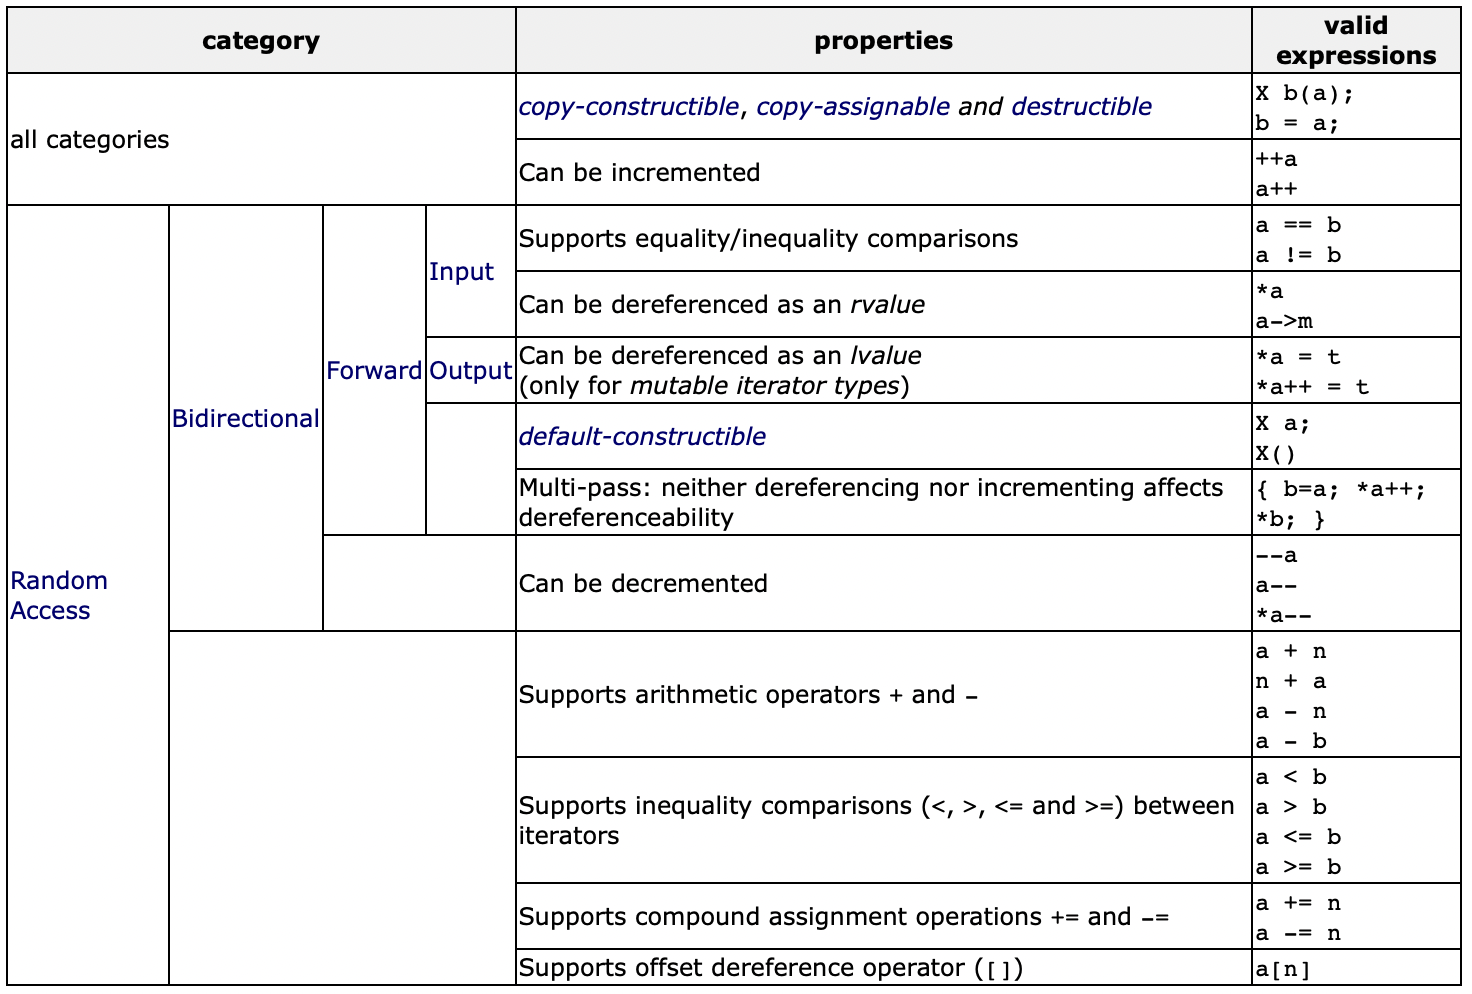
\includegraphics[height=8.5cm,keepaspectratio]{images/cpp-iters.png}
\end{center}
\end{frame}

% ----------------------------------------------------------------- %

\begin{frame}[fragile]
\frametitle{Iterators in C++}
Why we don't want this in Rust?

\begin{itemize}
    \item<1-> C++ iterators are universal, but their implementation totally violates the iterator concept, since you're actually iterating only in the case of ``Input iterator''.
    \item<2-> Since C++ is unsafe and don't have ownership like in Rust, they are always returning a reference, and moving object from the collection can be dangerous! But at the same time, almost all types of iterators allow that.
    \item<3-> It doesn't make sense to create traits for all types of ``iterators'' like in C++ since iterator should \textit{hide} details rather than \textit{expose} them, and moreover - it can give us misguided hopes.
\end{itemize}
\end{frame}

% ----------------------------------------------------------------- %

\begin{frame}[fragile]
\frametitle{Iterators in C++}
For instance, a list can also give us a random access iterator, but very inefficient. So, this code will compile but work extremely slowly:

\begin{minted}{cpp}
    template <class RandomIt>
    void func(RandomIt begin, RandomIt end) {
        // ...
        std::sort(begin, end);
        // ...
    }
\end{minted}

In Rust, you must know what collection you are using, and it's less error-prone.
\end{frame}

% ----------------------------------------------------------------- %

\end{document}
